\esSezione{Moltiplicatore di Booth su board}\label{sec:esercizio7-2}

\begin{traccia}
Sintetizzare il moltiplicatore implementato al punto~\ref{sec:esercizio7-1} su FPGA e testarlo mediante l'utilizzo dei dispositivi di input/output (switch, bottoni, led, display) presenti sulla board di sviluppo in dotazione. La modalità di utilizzo degli stessi è a completa discrezione degli studenti.
\end{traccia}

\progetto

Il moltiplicatore di Booth dell'esercizio~\ref{sec:esercizio7-1} viene istanziato così com'è in un nuovo top module, che si limita a collegarne le porte ai dispositivi della board. Non sono stati aggiunti componenti: il sistema è composto dalle sole entità già presentate (\texttt{booth}, \texttt{booth\_po}, \texttt{booth\_cu}, \texttt{add\_sub}, \texttt{rca}, \texttt{full\_adder}, \texttt{counter\_mod}), richiamate nei listati~\ref{lst:esercizio7-1:booth}, \ref{lst:esercizio7-1:booth-po}, \ref{lst:esercizio7-1:booth-cu}, \ref{lst:esercizio7-1:add-sub}, \ref{lst:esercizio7-1:rca}, \ref{lst:esercizio7-1:full-adder} e~\ref{lst:esercizio5-1:counter-mod}.

L'assegnazione dei dispositivi è la seguente:

\begin{itemize}
  \item i sedici switch forniscono gli operandi: \texttt{SW(15 downto 8)} per il moltiplicando \texttt{x} e \texttt{SW(7 downto 0)} per il moltiplicatore \texttt{y};
  \item il pulsante centrale \texttt{BTNC} è il segnale \texttt{start};
  \item il pulsante inferiore \texttt{BTND} è il segnale \texttt{rst};
  \item i sedici LED \texttt{LED(15 downto 0)} mostrano in binario il prodotto \texttt{p};
  \item il LED verde \texttt{LED16\_G} segnala il termine dell'operazione tramite \texttt{done}.
\end{itemize}

Si è scelto di non inserire debouncer né circuiti di visualizzazione su display: l'unità di controllo evolve a ogni fronte di salita del clock a \SI{100}{MHz} e sfrutta lo stato \texttt{S\_DONE}, nel quale resta finché \texttt{start} non torna a \texttt{'0'}. Il prodotto, in complemento a due, resta quindi stabile sui LED fino alla pressione successiva.

\implementazione

Il top module \texttt{booth\_tl} ha come porte il clock \texttt{CLK100MHZ}, il vettore \texttt{SW} a 16 bit, i pulsanti \texttt{BTNC} e \texttt{BTND}, il vettore \texttt{LED} a 16 bit e l'uscita \texttt{LED16\_G}. L'architettura \texttt{structural} contiene un'unica istanza, \texttt{Mbooth}, del componente \texttt{booth} (architettura \texttt{structural}), collegata con un port mapping diretto alle porte del top module.

\vhdlfile{esercizio7-2/booth_tl.vhd}{Implementazione del top module per la board}{lst:esercizio7-2:booth-tl}

Non è stato scritto un testbench specifico per questo top module, che non contiene logica propria.

\sintesiboard

Sulla scheda si impostano gli operandi con gli switch e si preme \texttt{BTNC}: la moltiplicazione parte e, alla conclusione degli otto passi, si accende \texttt{LED16\_G} mentre i LED \texttt{LED(15 downto 0)} riportano il prodotto a 16 bit. Rilasciando \texttt{BTNC} l'unità di controllo torna nello stato di attesa e una nuova operazione può essere avviata; \texttt{BTND} riporta il sistema alla condizione iniziale. % TODO: esiti della prova su board (foto/valori osservati) non disponibili

Nel file dei constraint sono state decommentate le seguenti righe.

\xdcfile{esercizio7-2/vincoli.xdc}{Constraint}{lst:esercizio7-2:vincoli}
\begin{figure}[H]
  \centering
  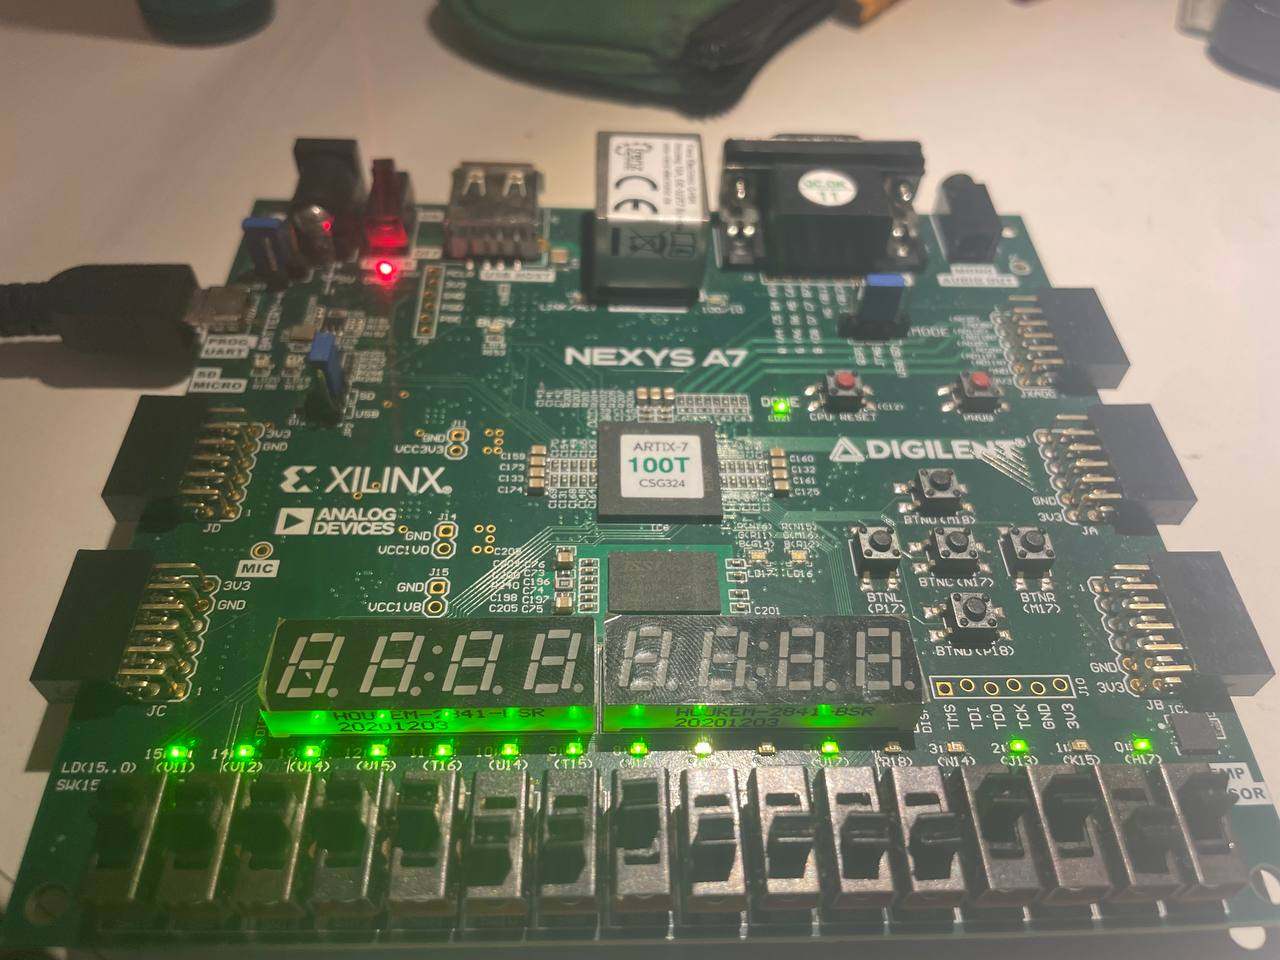
\includegraphics[width=\linewidth]{figure/esercizio7-2/irl.jpg}
  \caption{Realizzazione del moltiplicatore di Booth}
  \label{fig:esercizio7-2:booth}
\end{figure}